
\begin{figure}[H]
    \centering
    \pgfplotsset{
        % Configuración ajustada con más separación en Título y Eje X
        tight grid bar/.style={
            width=\linewidth,
            height=5.8cm,
            ybar,
            bar width=10pt,
            xlabel={Puntuación},
            ylabel={Número de votos},
            % Separación de etiquetas respecto al marco
            xlabel style={yshift=-0.2em},      % Aleja la etiqueta del eje X hacia abajo
            ylabel style={yshift=-0.6em},      % Mantiene el eje Y intacto
            title style={yshift=0.5em},        % Eleva el título hacia arriba
            % Elimina el margen exterior que reserva pgfplots para etiquetas
            trim axis left,
            trim axis right,
            nodes near coords, 
            nodes near coords align={vertical},
            every node near coord/.append style={
                font=\small,
                /pgf/number format/.cd, fixed, precision=0
            },
            enlarge x limits=0.08,
            enlarge y limits={upper, value=0.15}
        }
    }

    \begin{subfigure}{0.49\textwidth}
        \centering
        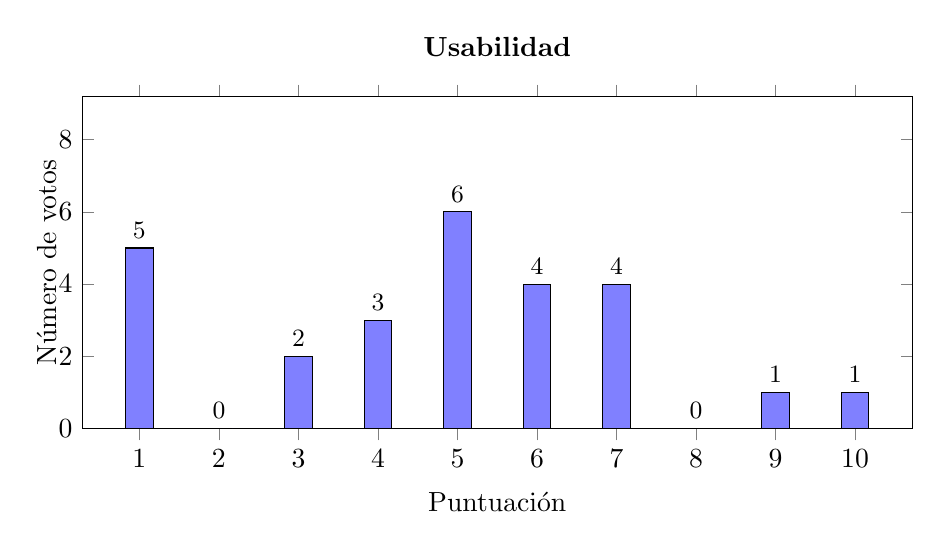
\begin{tikzpicture}
            \begin{axis}[
                tight grid bar,
                title={\textbf{Usabilidad}},
                ymin=0, ymax=8,
                ytick={0, 2, 4, 6, 8},
                xtick={1, 2, 3, 4, 5, 6, 7, 8, 9, 10},
                symbolic x coords={1, 2, 3, 4, 5, 6, 7, 8, 9, 10}
            ]
            \addplot[fill=blue!50] coordinates {
                (1, 5) (2, 0) (3, 2) (4, 3) (5, 6) (6, 4) (7, 4) (8, 0) (9, 1) (10, 1)
            };
            \end{axis}
        \end{tikzpicture}
    \end{subfigure}\hfill
    \begin{subfigure}{0.49\textwidth}
        \centering
        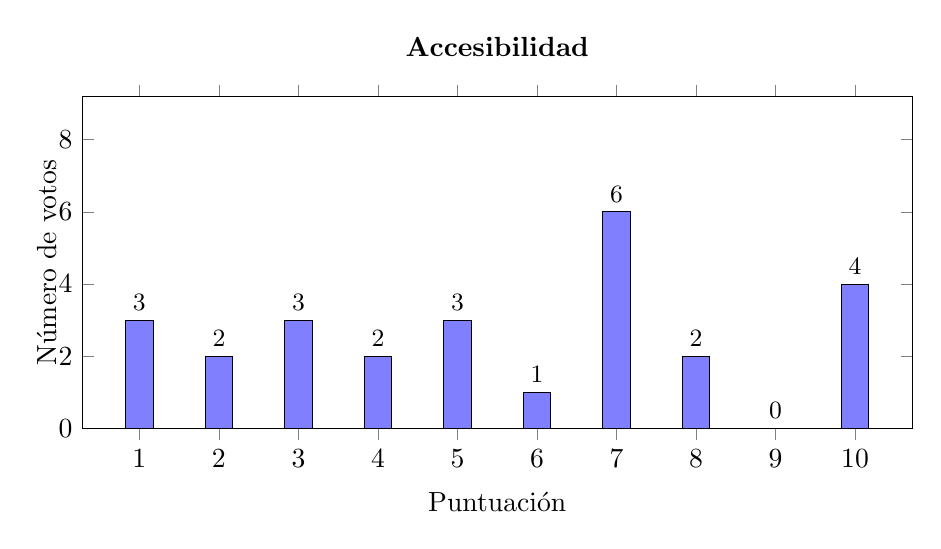
\begin{tikzpicture}
            \begin{axis}[
                tight grid bar,
                title={\textbf{Accesibilidad}},
                ymin=0, ymax=8,
                ytick={0, 2, 4, 6, 8},
                xtick={1, 2, 3, 4, 5, 6, 7, 8, 9, 10},
                symbolic x coords={1, 2, 3, 4, 5, 6, 7, 8, 9, 10}
            ]
            \addplot[fill=blue!50] coordinates {
                (1, 3) (2, 2) (3, 3) (4, 2) (5, 3) (6, 1) (7, 6) (8, 2) (9, 0) (10, 4)
            };
            \end{axis}
        \end{tikzpicture}
    \end{subfigure}

    \vspace{0.4cm} % Ligero incremento de separación entre filas por el desplazamiento del título inferior

    \begin{subfigure}{0.49\textwidth}
        \centering
        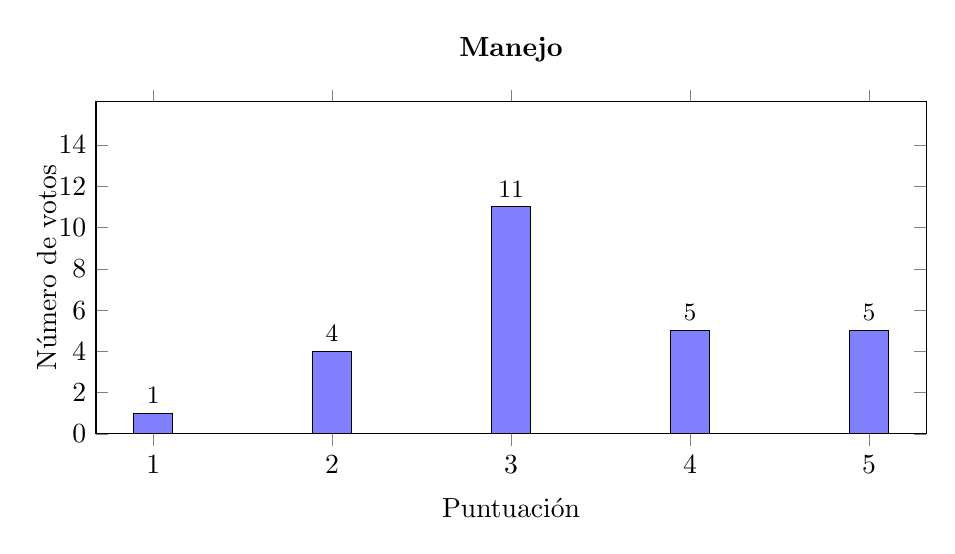
\begin{tikzpicture}
            \begin{axis}[
                tight grid bar,
                bar width=14pt,
                title={\textbf{Manejo}},
                ymin=0, ymax=14,
                ytick={0, 2, 4, 6, 8, 10, 12, 14},
                xtick={1, 2, 3, 4, 5},
                symbolic x coords={1, 2, 3, 4, 5}
            ]
            \addplot[fill=blue!50] coordinates {
                (1, 1) (2, 4) (3, 11) (4, 5) (5, 5)
            };
            \end{axis}
        \end{tikzpicture}
    \end{subfigure}\hfill
    \begin{subfigure}{0.49\textwidth}
        \centering
        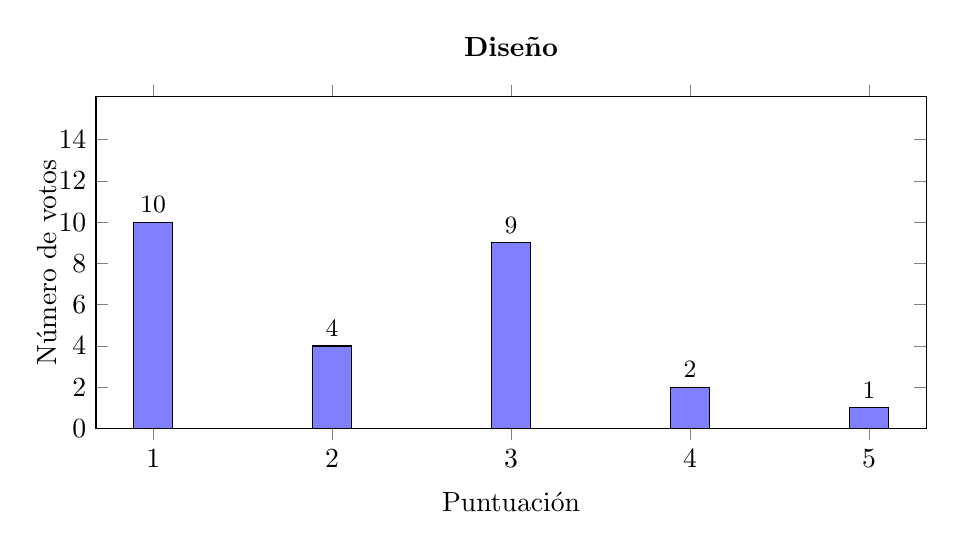
\begin{tikzpicture}
            \begin{axis}[
                tight grid bar,
                bar width=14pt,
                title={\textbf{Diseño}},
                ymin=0, ymax=14,
                ytick={0, 2, 4, 6, 8, 10, 12, 14},
                xtick={1, 2, 3, 4, 5},
                symbolic x coords={1, 2, 3, 4, 5}
            ]
            \addplot[fill=blue!50] coordinates {
                (1, 10) (2, 4) (3, 9) (4, 2) (5, 1)
            };
            \end{axis}
        \end{tikzpicture}
    \end{subfigure}

    \caption{Aspectos comunes}
    \label{fig:grid_common_aspects}
\end{figure}

Las cuatro gráficas de \ref{fig:grid_common_aspects} nos detallan cómo los usuarios sienten la interactividad con la aplicación. Esto nos puede ayudar a saber qué debemos cambiar respecto a la aplicación actual y qué podemos replicar y mejorar.

Podemos apreciar que a la mayoría de los usuarios no les desagrada la usabilidad. Con esto podemos intentar seguir un esquema de uso similar con el que cuenta la aplicación.

La accesibilidad parece seguir un patrón uniforme que crece conforme nos acercamos a valores que reflejan una menor accesibilidad. Lo que nos dice que la accesibilidad es un punto a mejorar necesitando crear un sistema intuitivo que no le genere fricción al usuario. 

El manejo es puntuado mayoritariamente con un valor medio, pero que decrece conforme nos acercamos a las mejores puntuaciones. Esto nos dice que necesitamos un sistema que ofrezca al usuario una distribución de los datos sencilla y entendible. 

Por último, el diseño no es puntuado muy alto, lo que nos dice que nuestro sistema deberá tener una mejora visual que sea atractiva para los usuarios.